\state{Generalized one-dimensional band theory}{
	Consider a 1D solid, lattice constant $a$, made of ``building blocks'' ($-a / 2< x < a / 2$) that scatter plane waves with a reflection coefficient $r$ and transmission coefficient $t$ ($\absr^2 + \abst^2 = 1$).  The energy of the plane wave is written as $\eps = \hbar^2 K^2 / 2 m$.  In the solid, the building blocks are stacked together indefinitely in the $x$ direction.
}

\prob{
	Write the solution to the {\Schrodinger} equation in the solid $\psix$ as a linear combination of $\psirx$ and $\psilx$, and use Bloch’s theorem to relate the wavefunction at each side of the building block (the same theorem applies to the gradient $\psi'$):
	\al{
		\psixpa &= e^{i k a} \psix, &
		\psipxpa &= e^{i k a} \psipx.
	}
	Hence, show
	\eq{
		\cos(k a) = \frac{t^2 - r^2}{2 t} e^{i K a} + \frac{1}{2 t} e^{-i K a}.
	}
}

\sol{
	Referring to the diagrams, we can write
	\al{
		\psilx &= \begin{cases}
			e^{i K x} + r e^{-i K x} & x \leq -\dfrac{a}{2}, \\[1ex]
			t e^{i K x} & x \geq \dfrac{a}{2};
		\end{cases}
		&
		\psirx &= \begin{cases}
			t e^{-i K x} & x \leq -\dfrac{a}{2}, \\[1ex]
			e^{-i K x} + r e^{i K x} & x \geq \dfrac{a}{2};
		\end{cases}
	}
	and the gradients
	\al{
		\psiplx &= \begin{cases}
			i K \paren{ e^{i K x} - r e^{-i K x} } & x \leq -\dfrac{a}{2}, \\[1ex]
			i K t e^{i K x} & x \geq \dfrac{a}{2};
		\end{cases}
		&
		\psiprx &= \begin{cases}
			-i K t e^{-i K x} & x \leq -\dfrac{a}{2}, \\[1ex]
			i K \paren{ -e^{-i K x} + r e^{i K x} } & x \geq \dfrac{a}{2}.
		\end{cases}
	}
	Inside the barrier,
	\al{
		\psix = A \psil + B \psir
		\quad
		-\frac{a}{2} \leq x \leq \frac{a}{2}.
	}
	Using Bloch's theorem \hl{(cite)}, we can write the boundary conditions~\cite[p.~147]{Ashcroft}
	\al{
		\psixpa &= e^{i k a} \psix, &
		\psipxpa &= e^{i k a} \psipx,
	}
	Imposing the first condition on the boundary at $x = -a / 2$, we find
	\al{
		 A t e^{i K a / 2} + B e^{-i K a / 2} + B r e^{i K a / 2} &= e^{i k a} \paren{ A e^{-i K a / 2} + A r e^{i K a / 2} + B t e^{i K a / 2} } \\
		B + (A t + B r) e^{i K a} &= e^{i k a} \brac{ A + (A r + B t) e^{i K a} } \\
		B \brac{ 1 + r e^{i K a} - t e^{i K a} e^{i k a} } &= A \brac{ e^{i k a} + r e^{i K a} e^{i k a} - t e^{i K a} } \\
		B &= e^{i k a} \frac{1 + r e^{i K a} - t e^{i K a} e^{-i k a}}{1 + r e^{i K a} - t e^{i K a} e^{i k a}} A.
	}
	Imposing the second gives us
	\al{
		i K \paren{ A t e^{i K a / 2} - B e^{-i K a / 2} + B r e^{i K a / 2} } &= i K e^{i k a} \paren{ A e^{-i K a / 2} - A r e^{i K a / 2} - B t e^{i K a / 2} } \\
		-B + (A t + B r) e^{i K a} &= e^{i k a} \brac{ A + (-A r + B t) e^{i K a} } \\
		B \brac{ -1 + r e^{i K a} + t e^{i K a} e^{i k a} } &= A \brac{ e^{i k a} - r e^{i K a} - t e^{i K a} e^{i k a} } \\
		B &= e^{i k a} \frac{1 - r e^{i K a} - t e^{i K a} e^{-i k a}}{-1 + r e^{i K a} + t e^{i K a} e^{i k a}} A.
	}
	Equating both expressions for $B$, we have
	\al{
		\frac{1 + r e^{i K a} - t e^{i K a} e^{-i k a}}{1 + r e^{i K a} - t e^{i K a} e^{i k a}} &= \frac{1 - r e^{i K a} - t e^{i K a} e^{-i k a}}{-1 + r e^{i K a} + t e^{i K a} e^{i k a}} \\
		\paren{ 1 + r e^{i K a} - t e^{i K a} e^{-i k a} } \paren{ -1 + r e^{i K a} + t e^{i K a} e^{i k a} } &= \paren{ 1 - r e^{i K a} - t e^{i K a} e^{-i k a} } \paren{ 1 + r e^{i K a} - t e^{i K a} e^{i k a} }.
	}
	The left side is
	\eq{
		-1 + r e^{i K a} + t e^{i K a} e^{i k a} - r e^{i K a} + r^2 e^{2i K a} + r t e^{2i K a} e^{i k a} + t e^{i K a} e^{-i k a} - r t e^{2i K a} e^{-i k a} - t^2 e^{2i K a},
	}
	and the right side is
	\eq{
		1 + r e^{i K a} - t e^{i K a} e^{i k a} - r e^{i K a} - r^2 e^{2i K a} + r t e^{2i K a} e^{i k a} - t e^{i K a} e^{-i k a} - r t e^{2i K a} e^{-i k a} + t^2 e^{2i K a}.
	}
	So the equality becomes
	\al{
		0 &= 1 - t e^{i K a} e^{i k a} - r^2 e^{2i K a} - t e^{i K a} e^{-i k a} + t^2 e^{2i K a} \\
		&= 1 - t e^{i K a} \paren{ e^{i k a} + e^{-i k a} } + (t^2 - r^2) e^{2i K a} \\
		&= 1 - 2 t e^{i K a} \cos(k a) + (t^2 - r^2) e^{2i K a}
	}
	or
	\eq{
		\ans{ \cos(k a) = \frac{t^2 - r^2}{2 t} e^{i K a} + \frac{1}{2 t} e^{-i K a} }
	}
	as we wanted to show. \qed
}



\prob{
	If the transmission coefficient is $t = \abst e^{i \del}$, it can be shown that $r = \pm i \absr e^{i \del}$.  Use this result to eliminate $r$ and show
	\eq{
		\frac{\cos(K a + \del)}{\abst} = \cos(k a).
	}
}

\sol{
	Feeding the coefficients and $1 = \abst^2 + \absr^2$ into the previous result, we have
	\al{
		\cos(k a) &= \frac{e^{2i \del} (\abst^2 + \absr^2)}{2 \abst e^{i \del}} e^{i K a} + \frac{1}{2 \abst e^{i \del}} e^{-i K a} \\
		&= \frac{e^{2i \del}}{2 \abst e^{i \del}} e^{i K a} + \frac{1}{2 \abst e^{i \del}} e^{-i K a} \\
		&= \frac{e^{i (\del + K a)}}{2 \abst} + \frac{e^{-i (\del + K a)}}{2 \abst} \\
		&= \ans{ \frac{\cos(K a + \del)}{\abst} }
	}
	as we wanted to show. \qed
}



\prob{
	Since $\abst < 1$, this result shows there are values of $K$ (and hence $\eps$) for which no Bloch states exist.  Demonstrate this by sketching the left-hand side as a function of $K$ (or preferably $\eps$).  Use your sketch to illustrate the behavior for
	\begin{enumerate}
		\item strong scattering, and
		\item weak scattering.
	\end{enumerate}
	Explain why, in general, electron bands tend to get wider and their gaps narrower as the electron energy increases.
}

\sol{
	\fig{13c}{
		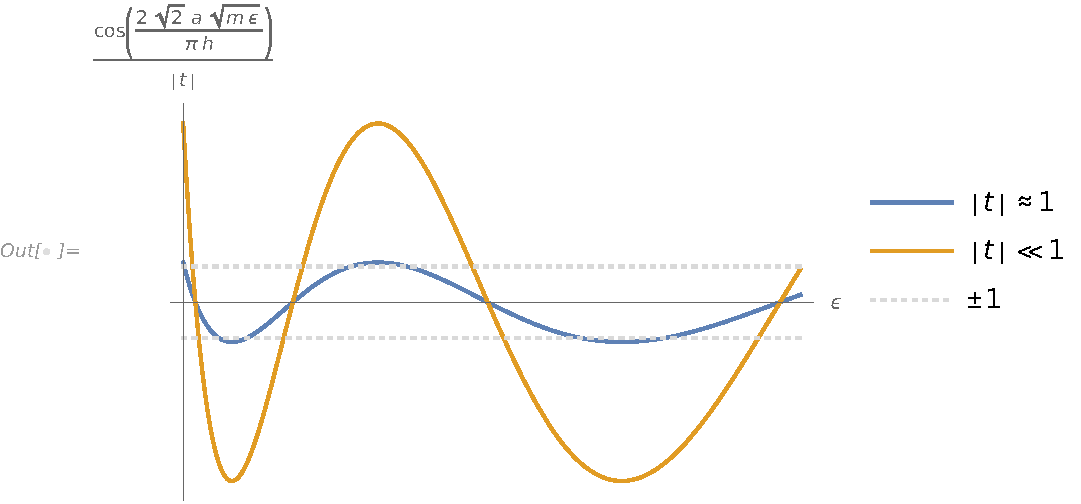
\includegraphics[width=0.6\textwidth,trim=1.5cm 0 0 0,clip]{13c}
		\caption{Plot of Eq.~\refeq{thing13c} with $\del = 0$ as a function of $\eps$.  Strong~(weak) scattering is shown as the blue~(gold) curve.  The ranges of $\eps$ for which the curves are between the light gray dashed lines are regions in which Bloch states exist.}
	}

	Figure~\ref{13c} shows
	\eqn{thing13c}{
		\frac{1}{\abst} \cos(\frac{a \sqrt{2 m \eps}}{\hbar} + \del)
	}
	as a function of $\eps$.  In the figure, the phase $\del = 0$.  No Bloch states exist in the regions in which
	\eq{
		\frac{\cos(K a + \del)}{\abst} > 1
		\qor
		\frac{\cos(K a + \del)}{\abst} < -1.
	}
	Strong scattering (blue curve) is associated with $\absr$ near 1 and small $\abst$, with the majority of the wave being being reflected.  Weak scattering (gold curve) is associated with small $\absr$ and $\abst$ near 1, with the majority of the wave being transmitted.  The regions with no existing Bloch states are narrower for strong scattering~\cite[p.~149]{Ashcroft}.
	
	This model suggests the electron bands and gaps both tend to widen as electron energy increases.  However, in general we expect the bands to widen and the gaps to narrow.  This is because the higher-energy atomic orbitals have larger radii; hence, there is a higher degree of overlap between high-energy orbitals of adjacent atoms than between low-energy orbitals of adjacent atoms.  As this degree of overlap increases, the degree of ``non-overlap'' decreases.  Since the bands represent the overlapping regions of space and the gaps represent the non-overlapping regions, the bands widen and the gaps narrow.
}